\documentclass[12pt]{article}

\usepackage{amsmath,amsthm,amssymb,xcolor,graphicx,tikz,listings}
\usepackage{comment}
\usepackage{cite}
\usepackage[utf8x]{inputenc}
\usepackage[pdftex]{hyperref}
\usetikzlibrary{positioning}

\begin{document}

% Macros
%------------------------------------------------------------
\def\Any {{\mathcal U}}
\def\Prop{{\mathcal P}}
\def\Indsort{{\Any_\mathcal I}}
\def\Fixsort{{\Any_\mathcal F}}
\def\Uni {{\mathcal L}}
\def\Univ {{\mathcal L}}
\def\Top {{\Box}}

\def\Nat{{\mathbb N}}

\def\case{{\text{\it case}}}
\def\ctree{{\text{\it tree}}}
\def\ct#1{{\mathcal #1}}
\def\cta {{\text{cta}}}
\def\fix {{\text{\it fix}}}
\def\fspinetree{{f_\text{st}}}
\def\llet{{\text{\it let}}}
\def\type{{\text{\it type}}}
\def\FV  {{\text{\it FV}}}

\def\Ind{{\cal I}}
\def\Make{{\cal M}}

\def\empty {\varepsilon}
\def\reduce{\leadsto}
\def\genreduce#1{\,\stackrel{#1}{\leadsto}\,}
\def\hreduce{\genreduce h}
\def\hstarreduce{\genreduce h^*}
\def\equiv {\,\sim\,}

%\def\meta#1{{{}^?\!\!#1}}
\def\meta#1{{{}^? \kern-0.2em #1}}
%\def\meta#1{{? \kern-0.2em #1}}
%\def\meta#1{{#1_?}}


\def\impl{\rightarrow}
%\def\vec#1{{\mathbf #1}}
\def\vec#1{{\overrightarrow {#1}}}
\def\fargs#1#2{{\vec {#1}^{\vec {#2}}}}

\def\set#1{{\{#1\}}}

\def\betaeq{{\stackrel \beta \sim}}


\def\brackets#1{\left[ {#1} \right]}
\def\parens#1{\left( {#1} \right)}

\def\ctreebr#1{{\ctree \brackets {#1}}}
\def\letbr#1{{\llet \brackets {#1}}}
\def\fixbr#1{{\fix  \brackets {#1}}}

\def\vertlist#1{
    \begin{array}{lllll}
    #1
    \end{array}
}

\def\bracklist#1{\brackets{ \vertlist{#1} }}


\def\cases#1{
    \left\{ \vertlist {#1} \right.
}


\def\rulev#1#2{
    \begin{array}{l}
        #1
        \\
        \hline
        #2
    \end{array}
}

\def\ruleh#1#2{
    \begin{array}{c}
        #1
        \\
        \hline
        #2
    \end{array}
}




% Put description label in italic (and not in bold)
\renewcommand{\descriptionlabel}[1]{\hspace{\labelsep}\textit{#1}}



\title{
    Compiling Alba
}

\author{
    Helmut Brandl
    \\
    \scriptsize (firstname dot lastname at gmx dot net)
}
\date{}

\maketitle


\abstract{
    How to compile Alba programs.
}


\tableofcontents

% Macros
%------------------------------------------------------------
\def\Any {{\mathcal U}}
\def\Prop{{\mathcal P}}
\def\Indsort{{\Any_\mathcal I}}
\def\Fixsort{{\Any_\mathcal F}}
\def\Uni {{\mathcal L}}
\def\Univ {{\mathcal L}}
\def\Top {{\Box}}

\def\Nat{{\mathbb N}}

\def\case{{\text{\it case}}}
\def\ctree{{\text{\it tree}}}
\def\ct#1{{\mathcal #1}}
\def\cta {{\text{cta}}}
\def\fix {{\text{\it fix}}}
\def\fspinetree{{f_\text{st}}}
\def\llet{{\text{\it let}}}
\def\type{{\text{\it type}}}
\def\FV  {{\text{\it FV}}}

\def\Ind{{\cal I}}
\def\Make{{\cal M}}

\def\empty {\varepsilon}
\def\reduce{\leadsto}
\def\genreduce#1{\,\stackrel{#1}{\leadsto}\,}
\def\hreduce{\genreduce h}
\def\hstarreduce{\genreduce h^*}
\def\equiv {\,\sim\,}

%\def\meta#1{{{}^?\!\!#1}}
\def\meta#1{{{}^? \kern-0.2em #1}}
%\def\meta#1{{? \kern-0.2em #1}}
%\def\meta#1{{#1_?}}


\def\impl{\rightarrow}
%\def\vec#1{{\mathbf #1}}
\def\vec#1{{\overrightarrow {#1}}}
\def\fargs#1#2{{\vec {#1}^{\vec {#2}}}}

\def\set#1{{\{#1\}}}

\def\betaeq{{\stackrel \beta \sim}}


\def\brackets#1{\left[ {#1} \right]}
\def\parens#1{\left( {#1} \right)}

\def\ctreebr#1{{\ctree \brackets {#1}}}
\def\letbr#1{{\llet \brackets {#1}}}
\def\fixbr#1{{\fix  \brackets {#1}}}

\def\vertlist#1{
    \begin{array}{lllll}
    #1
    \end{array}
}

\def\bracklist#1{\brackets{ \vertlist{#1} }}


\def\cases#1{
    \left\{ \vertlist {#1} \right.
}


\def\rulev#1#2{
    \begin{array}{l}
        #1
        \\
        \hline
        #2
    \end{array}
}

\def\ruleh#1#2{
    \begin{array}{c}
        #1
        \\
        \hline
        #2
    \end{array}
}




% Put description label in italic (and not in bold)
\renewcommand{\descriptionlabel}[1]{\hspace{\labelsep}\textit{#1}}


\lstdefinelanguage{alba}
{ basewidth=0.45em,
  basicstyle=\scriptsize\tt,  % choices: small, footnotesize, scriptsize, tiny
  mathescape,
  %columns=flexible,
  keywords={
    abstract,all,and,
    case,
    do,
    else,end
    ghost,
    if,in,inspect,
    let,
    mod,
    mutual,
    not,
    or,
    record,
    section,some,
    then,
    type,
    use,
    where,
    And,
    Not,
    Or
  },
  keywordstyle=\color{blue},
  commentstyle=\color{brown},
  morecomment=[l]{--},
  morecomment=[n]{\{-}{-\}}
}

\lstnewenvironment{alba} {\lstset{language=alba}} {}



\section{Universes}





\subsection{Universes and Sorts}


We have the following sorts or universes (sorts and universes are synonymous):
\begin{enumerate}
\item $\Prop$: Impredicative universe of propositions

\item $\Any_i$: Predicative universes of types for $i \in \set{0, 1, 2, \ldots}$

\item $\Any_\infty$: Top universe
\end{enumerate}
and the builtin type $\Uni$ with the typing judgements which are treated as
axioms:
$$
\begin{array}{l}
    \Uni : \Any_\infty
    \\
    \Prop : \Any_0 : \Any_1 \ldots
\end{array}
$$


All sorts except the top sort $\Any_\infty$ have types. Therefore it is
possible to introduce type variables $X: s$ for all sorts except the top sort.

Furthermore since $\Uni$ has type $\Any_\infty$ it is possible to introduce
universe variables $u: \Uni$.

The type of a type is always a sort. The sort of a type defines the
universe of the type. I.e. all types live in a universe. The typing judgement
$T: s$ says that the type $T$ lives in the universe $s$.


There is a subtle difference between the universe of a type and the universe of
an object. An object has a type and its type lives in a universe. We say the an
\emph{object $o$ lives in a universe $s$ if its type $T$ lives in the universe
$s$}. I.e. the typing judgement $o : T : s$ must be valid. In other words $o$
has type $T$ and $T$ has type $s$.

A type $T$ can be regarded as a type. Then its type is a sort $s$ with $T : s$
and it therefore lives in the universe $s$ as a type.

However a type can be regarded as an object as well. Then there is the typing
judgement $T: s_1 : s_2$. We say the object $T$ lives in the universe $s_2$.

Some examples: The type $\Nat$ lives in the universe $\Any_0$. The object $1$
has type $\Nat$. Therefore the object $1$ lives in the universe $\Any_0$. The
object $\Nat$ has type $\Any_0$ which has the type $\Any_1$. Therefore the
object $\Nat$ lives in the universe $\Any_1$. By the same reasoning the object
$\Any_0$ lives in the universe $\Any_2$.

All types regarded as objects live in a universe higher than the types regarded
as types.


Typing rules for products:
$$
\begin{array}{lll}
    \rulev{
        \Gamma \vdash A: s
        \\
        \Gamma, x^A \vdash B: \Prop
        \\
        A \ne \Uni
    }
    {
        \Gamma \vdash \Pi x^A. B : \Prop
    }
    &
    \rulev{
        \Gamma \vdash A: \Any_i
        \\
        \Gamma, x^A \vdash B: \Any_i
        \\
        A \ne \Uni
    }
    {
        \Gamma \vdash \Pi x^A. B : \Any_i
    }
    &
    \rulev{
        \Gamma \vdash u: \Uni
        \\
        \Gamma, u^\Uni \vdash B: s
        \\
        A \ne \Uni
    }
    {
        \Gamma \vdash \Pi u^\Uni. B : \Any_\infty
    }
\end{array}
$$
These rules guarantee that the type $\Pi u^\infty. B$ of a universe polymorphic
object cannot be used as an argument to a function.


\section{Bound Variables}

The function type

$$
\Pi x^A. R
$$

has a bound variable $x$ of type $A$ and a result type $R$ which might depend on
$x$.

A bound variable has the following attributes.

\begin{enumerate}

    \item Implicit: Let $f: \Pi x^A. R$ be a function and $f a$ an application.
        If the bound variable is implicit, then the compiler is instructed to
        infer the argument $a$ from the context in case it is missing.

        Implicit arguments are always ghost arguments. No runtime decisions and
        not runtime objects can be constructed by using implicit arguments.

    \item Type relevant: A variable is type relevant if the result type depends
        on it.

        Open point: What happens in
        $$
            \Pi P^{A \to \Any} x^A. P x
        $$
        if $P = \lambda x^A . N$? Is $x$ type relevant?

    \item Ghost: A ghost variable means that its value cannot be used in the
        runtime code. It can be

        \begin{itemize}
            \item used in types

            \item used as an argument to a function which expects a ghost argument

            \item pattern matched on to make decisions if the result type of the
                decision is a proposition

            \item used as an argument to any function whose return type is a
                propositon.

        \end{itemize}
\end{enumerate}

A type is a proposition or a propositional type if its type is $\Prop$. All
other types are non propositional types. Any term whose type is a proposition is
a proof of the proposition. All terms whose type is a proposition are ghost
terms because they are never runtime objects.


There are the following rules:

\begin{enumerate}
    \item All type relevant arguments in a global function whose type is a
        proposition are mandatory implicit. If the function is not global, then
        the argument can be implicit or not.

    \item All type relevant arguments whose type is not a
        proposition can be declared implicit or not.

        If declared implicit, then they are ghost variables. This implies that
        the function is not allowed to make any runtime decisions or construct
        any runtime objects using the ghost argument. Ghost arguments are only
        available at compile time.

    \item If a non-ghost function is fed with a ghost argument where it expects
        a non-ghost argument (i.e. an explicit argument), then the result is
        infected i.e. the result is converted to a ghost object.

    \item An argument which is not type relevant is not allowed to be implicit.
\end{enumerate}


If a constructor for a proposition uses non-propositional bound variables, then the
non-propositonal bound variable is a ghost variable. A pattern match uncovering
it can use its value only as a ghost value. A decision cannot be made on pattern
match unless the result type of the pattern match is a proposition.


\section {Inductive Types}


\subsection{Form of an inductive type:}
%--------------------------------------------------------------------------------


$$
    \type_i[\Gamma, \vec {X^K := \vec C}]
$$

\begin{description}
    \item [Parameters $\Gamma$] Context of parameters. It binds all free
        variables in the kinds and the constructurs.

    \item [Kinds $K_i$] The have the form $\Pi \vec {x^A}. s$ of a function
        type.
        Kinds have an arity which is possibly zero and a sort $s$ as its
        result type.

    \item [Constructor types $C_{i \ell_j}$] Each constructor type has a label.
        All labels for the same $i$ must be different. The constructor types
        have the form
        $$
            \Pi \Delta. X_i \vec a
        $$
        where the context $\Delta$ might be empty and all $X_j$ can occur in
        $\Delta$ only positively i.e. $\Delta$ has the structure
        $$
            [y_1^{\Pi B_1. R_1}, \ldots, y_n^{\Pi B_m. R_m}]
        $$
        and $X_j$ can occur only in $R_i$ and if it occurs in $R_i$, then $R_i$
        has the form $X_j \vec a$. I.e. the arguments of constructors are
        functions (arity zero included) where $X_j$ occurs only in the result type
        and not in the argument types.

    \item [Recursive]
        An inductive type is recursively defined if $X_j$ occurs in the result
        type of any constructor argument.
\end{description}


\begin{alba}
    type Nat: Any :=
        zero: Nat
        succ: Nat -> Nat


    type (<=): Nat -> Nat -> Prop
    :=
        z<=n {n}: zero <= n
        s<=s {n m}: n <= m -> succ n <= succ m


    mutual (A: Any)
        type Tree: Any :=
            node: A -> Forest -> Tree

        type Forest: Any :=
            []: Forest
            (::): Tree -> Forest -> Forest


    type Acc {A: Any} (R: A -> A -> Prop): A -> Acc
    :=
        acc {x}: (all {y}: R y x -> Acc y) -> Acc x


    type (=) {A: Any}: A -> A -> Prop
    :=
        refl {x}: x = x
\end{alba}


\paragraph{Implementation Hints}
\begin{enumerate}
    \item Since the result type of a constructor must always have the form $X
        \vec a$ it is not necessary to store the whole expression. It is
        sufficient to store the index arguments $\vec a$.

        \begin{alba}
            type Nat: Any :=
                zero: _
                succ: Nat -> _

            type (<=): Nat -> Nat -> Prop
            :=
                z<=n {n}: _ zero n
                s<=s {n m}: n <= m -> _ (succ n) (succ n)
        \end{alba}

    \item The kinds must have the form $\Pi \vec{x^A}. s$. It is sufficient to
        store the array of the index arguments $\vec {x^A}$ and the sort.

    \item The constructor types have the form $\Pi \vec{y^D}. X_i \vec a$. The
        constructor arguments $\vec {y^D}$ can be stored as an array (i.e. a
        context). If any $X_j$ occurs in a type of a constructor argument
        (recursive case), then
        it can occur only as a result type. The non recursive argument types can
        be stored just as a normal term. The recursive argument types can be
        stored as an array plus the result type.

    \item Parameters of type $\Prop$ or $\Any$ can generate nested inductive
        types (e.g. {\tt List (Tree A)}). Therefore it might be interesting to
        check, if a type variable occurs only positively in constructor
        arguments.
\end{enumerate}




\subsection{Examples}
%--------------------------------------------------------------------------------
$$
    \begin{array}{lll}
        \text{boolean}
        &
        \type[B^\Any \mid B, B]
        \\
        %
        \text{peano numbers}
        &
        \type[N^\Any \mid N, N\to N]
        \\
        %
        \text{list}
        &
        \type[A^\Any \mid L^\Any \mid L, A \to L\to L]
        \\
        %
        \text{equality}
        &
        \type[A^\Any
        \mid E^{A \to A \to \Prop}
        \mid \Pi x^A. E x x]
        \\
        %
        \text{accessibles}
        &
        \type[
            A^\Any, R^{A \to A \to \Prop}
            \mid
            T^{A \to \Prop}
            \mid
            \Pi x^A. (\Pi y^A. R y x \to T y) \to T x
        ]
    \end{array}
$$

In peano numbers the first constructor type has no arguments. The second has one
recursive argument.




\subsection{Constructors}
%--------------------------------------------------------------------------------

$$
    \Make^\Ind_{\ell_i} \vec p \vec b: \Ind \vec p \vec a
$$
where $\Ind$ is the inductive type, $i$ marks the $i$th constructor, $\vec p$ are
the parameter arguments and $\vec b$ are the constructor arguments, $a$ are the
index arguments which depend on the constructor arguments.

The peano number $2$ looks like $ \Make^N_1 (\Make^N_1 \Make^N_0) $.

A constructor has the type
$$
    \Make^\Ind_{\ell_i} : \Pi \Gamma \Delta_{\ell_i}. T {\vec a}_{\ell_i}
$$





\subsection{Typing}
%--------------------------------------------------------------------------------

Let $\Ind = [\Gamma \mid T^K \mid C_{\ell_1}, \ldots, C_{\ell_n}]$ be a wellformed
inductive type. Then we have the following typing rules.

\begin{description}

    \item [Inductive type]
        $$
            \rulev{
                K \; \betaeq\; \Pi \Gamma_K. s
                \\
                \forall i.\; \Gamma, T^K \vdash C_{\ell_i}: s
            }
            {
                [] \vdash \Ind : \Pi \Gamma. K
            }
        $$


    \item [Constructor] Let $C_{\ell_i} = \Pi \Delta. T \vec a$.
        $$
        \rulev{
            [] \vdash \Ind: \Pi \Gamma. K
        }
        {
            \Make^\Ind_{\ell_i}: \Gamma \Delta.T \vec a
        }
        $$
\end{description}






\subsection{Mutually defined Inductive Types}
%--------------------------------------------------------------------------------

It is just an array of inductive types where all inductive types share the same
parameters.
$$
    \type
    \left[\Gamma \mid
    \bracklist{
        T_1^{K_1} \mid C_{11}, \ldots, C_{1n_1}
        \\
        \ldots
        \\
        T_m^{K_m} \mid C_{m1}, \ldots, C_{mn_m}
    }
    \right]
$$

All kinds $K_i$ are valid in the context $\Gamma$ and all constructors of the
$i$th type construct an object of type $T_i \vec a$ but can use any other
objects of type $T_j \vec a$ as arguments. All constructors are valid types in
the context $\Gamma, T_1^{K_1}, \ldots , T_m^{K_m}$.


{
    \def\ct{f_\text{ct}}

    \section{Pattern Match}
%----------------------------------------------------------------------

\subsection{Basics}
%----------------------------------------------------------------------

Fully elaborated pattern match expression:
$$
\case[ f^F \mid c_1,  \ldots, c_n \mid t]
$$
%
where $F$ is a function type of the form
%
$$
\Pi x_1^{A_1} \ldots x_k^{A_k}. R
$$
%
and where each clause $c_i$ has the form
%
$$
    [\Delta \mid p_1^{P_1}, \ldots, p_m^{P_m} \mid e^E]
$$
where the context $\Delta$ contains all pattern variables introduced in the
pattern, $p_i$ is the $i$-th pattern
and $P_i$ is the corresponding type of the pattern, $e$ is the body of the
clause, $E$ its corresponding type and $t$ is a case tree (see below).

Each clause defines the function
$$
\lambda \Delta . e^E
$$


The patterns are terms generated from the grammar
$$
    p ::= x \mid x := c \mid x := \Make^I_\ell \vec q \vec p
$$
where $c$ ranges over constants (strings, characters, numbers, etc.), $x$ ranges
over variables and $p$ ranges over pattern. The expression $\Make^I_\ell \vec q
\vec p$ is the constructor with label $\ell$ of the inductive type $I$ applied to its
parameter arguments and to its arguments.

Patterns are trees. Each node of the tree is labelled by a pattern variable and
either by a constant or a constructor $\Make^I_\ell \vec q$. A pattern clause has a
sequence of trees.

The pattern variables are assumed to be distinct in all clauses.



\subsection{Welltyped}
%------------------------------------------------------------

A clause of the pattern match expression is welltyped if
$$
\begin{array}{lll}
    \Delta &\vdash& p_i : P_i
    \\
    \Delta &\vdash& e : E
\end{array}
$$
%
and
%
$$
\begin{array}{lll}
    P_i &\le& A_i[p_1,\ldots,p_{i-1} / x_1,\ldots,x_{i-1}]
    \\
    E   &\le& R[p_1,\ldots,p_m / x_1,\ldots,x_m]
\end{array}
$$
%
where $F = \Pi x_1^{A_1} \ldots x_m^{A_m}. R$.




\subsection{Syntactical Pattern}
%------------------------------------------------------------

The pattern in the source code are generated from the grammar
$$
\begin{array}{llll}
    p_s
    &:=&   x                   & \text{pattern variable}
    \\
    &\mid& \ell \vec p_s       & \text{constructor + arguments}
    \\
    &\mid& c                   & \text{constant}
    \\
    &\mid& x := \ell \vec p_s
    \\
    &\mid& x := c
\end{array}
$$


A constructor label $\ell$ without arguments and a variable name $x$ are
indistiguishable in the source code. They are just names. But since the required
type is known it is clear if the name is one of the labels of the corresponding
inductive type. In that case the name is a label and not a pattern variable.






\subsection{Case Tree}
%------------------------------------------------------------

A case expression is a function which can be applied to arguments
$$
    \case[\ldots] a_1 \ldots a_n
$$
%
The task of a valid case tree is to
\begin{itemize}
    \item split the arguments into a series of subterms $u_1,u_2, \ldots$

    \item decide which case clause is applicable (if sufficient information is
        available)

    \item return the result $e[u_1, u_2, \ldots / .]$ where $e$ is the right
        hand side of the applicable case clause.
\end{itemize}

A case tree is defined by the grammar

$$
    \begin{array}{lllll}
        t
        &::=& e
        %
        \\
        &\mid& [x^T \mid t]
        %
        \\
        &\mid& [
            x^T
            \mid
            c_1 t_1, \ldots,  c_n t_n \mid
            \ell_1 t_1, \ldots, \ell_m t_m
            \mid
            d
        ]
    \end{array}
$$
%
where $n + m > 0$ and
%
\begin{center}
    \begin{tabular}{l p{8cm}}
        $t$ & case tree
        \\
        $d$ & optional case tree (default or catch all)
        \\
        $e$ & expression on the right hand side of a case clause
        \\
        $x^T$ & pattern variable with its corresponding type
        \\
        $c$ & constant
        \\
        $\ell$ & label of a constructor
    \end{tabular}
\end{center}

We can abbreviate the second form of an inner node by $[x^T \mid \vec c\vec t \mid
\vec\ell \vec t | d]$.


No duplicate constants and no duplicate labels are allowed in the second form of
an inner node.

The application of a case scans the list of arguments left to write with a
pointer to a subexpression to some of its arguments. Semantic actions associated
to the nodes of a case tree.
\begin{itemize}
    \item $e$: The pointer has to point beyond the last argument of the
        arguments. The list of collected subexpression $u_1, u_2, \ldots$ cover
        all free variables in the expression $e$. Action: Return the value
        $e[u_1,u_2,\ldots / .]$.

    \item $[x^T \mid t]$: The pointer has to point to some subexpression of the
        arguments and there has to be a next pointer position. Action: Append
        the term $u$ to the list of terms $u_1,u_2,\ldots$ where $u$ is the
        subexpression at the pointer and apply the case tree $t$ to the pointer
        advance by one.

    \item $[x^T \mid \vec c \vec t \mid \vec \ell \vec t \mid d]$:
        The pointer has to point to some subexpression of the arguments. The
        subexpression has to reduce to a head normal form which has either a
        constant or a constructor in the head position. From the constant or the
        constructor it is clear which case tree is the next to apply.
        Actions:
        \begin{itemize}
            \item Append the subexpression to the list $u_1,u_2,\ldots$.

            \item If the default tree is the next tree then apply it to the next
                pointer position.

            \item If the subexpression is a constant then apply the
                corresponding next tree to the next pointer position.

            \item If the subexpression is a constructor without index
                arguments then apply the corresponding next tree to the next
                pointer position.

            \item If the subexpression is a constructor with arguments then
                apply the corresponding next tree to the pointer pointing at the
                first index argument of the constructor (skip the parameter
                arguments).
        \end{itemize}
\end{itemize}



\paragraph{Exhaustiveness of inner nodes}
%

An inner node of the form $[x^T \mid \vec c \vec t \mid \vec\ell \vec t \mid d]$ is
exhaustive if it has a default tree or if all labels of constructors which can
construct an object of the corresponding type are present (none of the missing
constructors can construct an object of type $T$).

An empty inner node of the form $[x^T \mid \empty \mid \empty \mid \empty]$ is
possible if $T$ is an inductive type and none of the constructors of the
inductive type can construct an object of type $T$.

\paragraph{Exhaustiveness of a case tree}
%
A case tree is exhaustive if all its nodes are exhaustive.



\paragraph{Redundancy of an inner node}

An inner node of the form $[x^T \mid \vec c \vec t \mid \vec\ell \vec t \mid d]$
is redundant if
\begin{itemize}
    \item it has multiple entries of the same constant

    \item it has multiple entries of the same constructor

    \item it has a default tree and none of the missing constructors can
        construct an object of type $T$ or there are no missing constructors.
\end{itemize}



\paragraph{Redundancy of case tree}

A case tree is redundant of some of its nodes are redundant.




\subsection{Case Tree Construction}
%------------------------------------------------------------

\paragraph{Case tree for a clause}
First we construct a case tree from a cause clause
$\Delta \vec p^{\Vec p} := e$.

$$
\begin{array}{lll}
    \ct(\Delta \vec p^{\vec P} := e) &:=& \ct(\vec p, e)
    \\
    \ct(x, t) &:=& [x \mid t]
    \\
    \ct(x := c, t) &:=& [x \mid c\, t \mid \epsilon ]
    \\
    \ct(x := \Make^I_\ell \vec q \vec p, t)
                   &:=&
                   [x \mid \ell\, \ct(\vec p, t) \mid \epsilon ]
\end{array}
$$
%
where $\ct(\vec p, t)$ on a sequence of pattern is threaded from behind
%
$$
\ct(p_1 \ldots p_{n-1} p_n, t)
:=
\ct(p_1, (\ldots \ct(p_{n-1}, \ct(p_n, t))\ldots))
$$


Note that the case tree of a cause clause has no branching and no default trees.
It is a path from the root to a leave.



\paragraph{Merge case trees} We have to be able to merge two case trees $t_1$
and $t_2$ to $m(t_1, t_2)$ where the first one might be empty and the second one
has been constructed from a clause of the pattern match expression.

$$
\begin{array}{lll}
    m(\varepsilon, t)
    &:=&
    t
    \\
    m([x \mid \ldots], e)
    &:=&
    m([x \mid \ldots], [x \mid e]))
    \\
    m([x \mid t], [x_2 \mid t_2])
    &:=&
    [x \mid m(t, t_2[x/x_2])]
    \\
    m([x \mid t], [x_2 \mid c_2 t_2 ])
    &:=&
    ??
    \\
    m([x \mid \vec c \vec t \mid \vec \ell \vec t \mid d], [x_2 \mid t_2])
    &:=&
    \begin{array}[t]{@{}l}
        [x
        \\
        \mid m(\vec c \vec t, t_2[x/x_2])
        \\
        \mid m(\vec \ell \vec t, t_2[x/x_2])
        \\
        \mid m(d, t_2[x/x_2])
        ]
    \end{array}
    \\
    m([x \mid \vec c \vec t \mid \varepsilon \mid d],
        [x_2 \mid c_2 t_2 \mid \varepsilon])
    &:=&
    [x \mid m(\vec c \vec t, c_2 t_2[x/x_2]) \mid \varepsilon \mid d]
    \\
    m([x \mid \vec c \vec t \mid \vec \ell \vec t \mid d],
        [x_2 \mid \ell_2 t_2 \mid \varepsilon])
    &:=&
    [x \mid \vec c \vec t \mid m(\vec \ell \vec t, \ell_2 t_2[x/x_2]) \mid d]
    \\
    m(\vec c \vec t, c_\text{new} t_2)
    &:=&
    \vec c \vec t c_{\text{new}} t_2
    \\
    m(\vec \vec \ell \vec t, \ell_\text{new} t_2)
    &:=&
    \vec \ell \vec t \ell_{\text{new}} t_2
    \\
    m(\ldots ct \ldots, c t_2)
    &:=&
    \ldots c m(t,t_2) \ldots
    \\
    m(\ldots \ell t \ldots, \ell t_2)
    &:=&
    \ldots c m(t,t_2) \ldots
\end{array}
$$
%
where $m(\vec c \vec t, t_2)$ and $m(\vec \ell \vec t, t_2)$ means that $t_2$ is
merged into all trees $\vec t$.

The missing cases are error cases.
%
\begin{enumerate}
    \item $m(e, t)$: The tree $t$ is redundant. It cannot add any new decisions.

    \item $m([x \mid t], [x_2 \mid c_2 t_2 ])$: The clauses are out of order. A
        catch all pattern cannot be followed by a more specific pattern. If it
        were allowed the more specific pattern could shadow cases treated by the
        catch all pattern.

    \item $m([x \mid t], [x_2 \mid \ell_2 t_2 ])$: Same as before.
\end{enumerate}


\paragraph{Algorithm}

\begin{enumerate}
    \item Start with an empty case tree.

    \item For all clauses: Construct a case tree from the clause and merge it
        into the existing case tree.

    \item Stop at the last clause or as soon that a clause can add nothing to a
        case tree. A clause which can add nothing is redundant which is
        considered as an error.
\end{enumerate}







\subsection{Exhaustiveness and Redundancy}
%------------------------------------------------------------

\emph{Focal point}
Each pattern in a pattern clause can be regarded as a focal
point. At the focal point we have either a variable, a constructor pattern or a
constant. The focal point of two consecutive clauses is the first pattern where
both clauses have a different pattern (we do not regard $p$ and $x:=p$ as
different).

If two consecutive clauses don't have a focal point, then the second one is
redundant which is regarded as an error (the clause is unreachable).








\subsection{Application of a pattern match expression}

An application of a pattern match expression (whose type is always a function
type) has the form
$$
\case(f^F, \vec c) \vec a
$$
where $\vec a = [a_1, \ldots, a_n]$ are the arguments to which the pattern match
function is applied. The maximal number of arguments is determined by the type
$F$ of the pattern match expression.

The application can be evaluated if it is possible to find a clause of the
pattern match expression and split the arguments $\vec a$ into subexpressions
$\vec s$ and evaluate $(\lambda \Delta. e^E) \vec s$.

A pattern match expression applied to arguments is a reducible expression
$$
\case(f^F, \vec c) \vec a \quad\to\quad e[case(f^F, \vec c), \vec s / f, \vec x]
$$
where $e$ is the expression on the right hand side of the found clause, $\vec x$
are the pattern variables of this clause and $\vec s$ are the subexpressions
extracted from the arguments $\vec a$ during walking down the case tree. The
hole case expression is substituted for the variable $f$ representing the
function and the subexpressions $\vec s$ are substituted for the pattern
variables $\vec x$.



\subsection{Code Examples}
%----------------------------------------------------------------------



\paragraph{Unbounded Loop}

\ \begin{alba}
    section
        P: Nat -> Prop
        d: Decider P
        e: Exist P
    :=
        type R: Nat -> Nat -> Prop :=
                -- 'n' and its successor figure in the relation 'R'
                -- if 'n' does not satisfy the predicate.
            next {n}: not P n -> R n (succ n)

        type Via: Nat -> Prop :=
                -- Set of viable candidates: A number 'n' is in the
                -- set if all its successors in the relation 'R' are
                -- in the set.
            via {x}: (all {y}: R x y -> Via y) -> Via x

        stepDown {n} (v: Via (succ n)): Via n :=
            via {n} f where
                f: all {m}: R n m -> Via m
                := case
                    \ next _ : Via (succ n) := v
\end{alba}


\paragraph{Vector}

\ \begin{alba}
    type Vec (A: Any): Nat -> Any :=
        []:  Vec zero
        (::) {n: Nat}: A -> Vec n -> Vec (succ n)

    zip {A B: Any}
    : all {n}: Vec A n -> Vec B n -> Vec (A,B) n
    := case
        \ nil,     nil     := nil
        \ x :: xs, y :: ys := (x, y) :: zip xs ys
\end{alba}

\begin{alba}
    map {A B C} (f: A -> B -> C)
        : all {n}
          : Vec A n -> Vec B n -> Vec C n
    := case
        \ {zero},   [],            [] :=
            []
        \ {succ n}, (::) {n} x xs, (::) {n} y ys :=
            (::) {n} (f x y) (map {n} xs ys)
        -- without implicits
        \ [] []            := []
        \ x :: xs, y :: ys := (f x y) (map xs ys)
\end{alba}





\paragraph{Less Equal on natural numbers}


\ \begin{alba}
    type (<=): Nat -> Nat -> Prop :=
        start {n}:    0 <= n
        next  {n m}:  n <= m -> succ n <= succ m

    leRefl: all {n: Nat}: n <= n := case
        \ {zero}   := start {zero}
        \ {succ n} := next {n} {n} (leRefl {n})

        -- without implicits
        \ {zero}   := start
        \ {succ n} := next leRefl
\end{alba}

Pattern match on implicits is allowed in this case, because the result type is a
proposition!




\paragraph{Equality}

\ \begin{alba}
    type (=) (A: Any): A -> A -> Prop :=
        same {x}: x = x

    zeroNeSucc: all {n: Nat}: zero = succ n -> False :=
        case
            -- no case clauses
\end{alba}

The compiler has to verify that no match is possible. The pattern match
expression is the two argument function with type $\Pi n^N. 0 = 1 + n \to
\text{False}$.



\paragraph{$<=?$}
\ \begin{alba}
    type Nat := [zero, succ: Nat -> Nat]

    (<=?): Nat -> Nat -> Nat := case
        \ zero,   _      :=  true
        \ succ _, zero   :=  false
        \ succ n, succ m :=  n <=? m

    -- as case tree:
    case
        zero           :=   \ _ := true
        succ n :=
            case
                zero   :=   false
                succ m :=   n <=? m
\end{alba}


\paragraph{Parity}
\ \begin{alba}
    type Parity: Nat -> Any :=
        even n: Parity (n + n)
        odd  n: Parity (succ (n + n))

    parity: all n: Parity n := case
        \ zero: Parity zero :=
            even
        \ succ n: Parity (succ n) :=
            match parity n case
                \ even nh :=
                    odd nh
                \ odd nh :=
                    even (succ nh)

    natToBin: Nat -> List Bool := case
        \ zero :=
            []
        \ succ n :=
            match parity n case
                \ even nh :=
                    false :: natToBin nh
                \ odd nh :=
                    true :: natToBin nh
\end{alba}

}

\section{Elaboration}
%--------------------------------------------------------------------------------







\subsection{Basics}
%--------------------------------------------------------------------------------

After parsing we get an abstract syntax tree (AST) of the source file. Each
subterm of the AST gets a source based metavariable, a goal and a task which
elaborates the source term. Source based metavariables are never instantiated by
constraint solving. Source based metavariable are instantiated at the end of the
corresponding task.

The elaborator can create more metavariables for the following reasons:

\begin{enumerate}
    \item Missing type information in the source code.

    \item Implicit function arguments not explicitly provided in the source code.

    \item Wild cards in the source code (the wild card {\tt \_} is a request
        from the programmer to the compiler to fill in the information).

    \item Intermediate metavariables introduced during unification for subterms
        in an imitation step where the pattern on flex side include variables
        regarded as constants.

    \item Pattern variables in case trees.
\end{enumerate}

The instantiation of metavariables is used to synchronize the tasks in the
elaborator. A task can be blocked because it is waiting for one or more
metavariables to be instantiated (e.g. when the metavariable is the head term
and head normal form is required). A task which instantiates a metavariable
unblocks all tasks which wait for the instantiation of the metavariable.

Finally either all metavariables are instantiated or a deadlock is reached
because the wait-for graph has become cyclic.

The wait-for graph for source based metavariables can never become cyclic
because source based metavariables have a clear hierarchy given by the AST.
Therefore if the programmer provides all type information and all implicit
arguments explicitly a dead lock can never
appear. A deadlock appears if the compiler cannot elaborate the missing
information.

Metavariables representing missing information must have enough source code
information to generate a useful error message. If a deadlock occurs, the
elaborator searches for the first metavariable representing missing
information and prints an error message.






\subsection{Definitions}
%--------------------------------------------------------------------------------

$$
\Gamma
\vdash
f
    \underbrace{
        x_0^{A_0} \ldots x_{n-1}^{A_{n-1}}
        }_{\text{parameter args}}
    :
    \Pi
        \underbrace{
            x_n^{A_n} \ldots x_{n+m-1}^{A_{n+m-1}}
        }_{\text{index args}}
    .
    R
    := e
$$
with $n$ parameter arguments and $m$ index arguments.


\begin{enumerate}

    \item
        Introduce the metavariables
        $$
        \vertlist{
            \meta u &:& \Univ
            \\
            \meta A_0 &:& \Any_{\meta u}
            \\
            \meta A_1 &:& \Pi x_0^{\meta A_0}. \, \Any_{\meta u}
            \\
            \meta A_2 &:& \Pi x_0^{\meta A_0} x_1^{\meta A_1 x_0}. \,
            \Any_{\meta u}
            \\
            \ldots
            \\
            \meta R
            &:&
            \Pi
                x_0^{\meta A_0}
                \ldots
                x_{n+m-1}^{\meta A_{n+m-1} x_0 x_1 \ldots x_{n+m-2}}
            . \, \Any_{\meta u}
            \\
            \meta e_0
            &:&
            \Pi \vec {x^A}. R
            \\
            \meta e_1
            &:&
            \meta R x_0 x_1 \ldots x_{n+m-1}
        }
        $$
        and the contexts
        $$
        \vertlist{
            \Gamma_0 &=& \Gamma
            \\
            \Gamma_1 &=&
                \Gamma, x_0^{\meta A_0}
            \\
            \Gamma_2 &=&
                \Gamma, x_0^{\meta A_0}, x_1^{\meta A_1 x_0}
            \\
            \ldots
            \\
            \Gamma_{n+m-1} &=&
                \Gamma,
                    x_0^{\meta A_0},
                    x_1^{\meta A_1 x_0},
                    x_2^{\meta A_2 x_0 x_1}
                    \ldots
        }
        $$
        For each type which has source code the metavariables are source based.
        The remaining metavariables have to be resolved by constraint solving.

        All metavariables for the types are introduced in the context $\Gamma$.
        Therefore it is possible to assign to the variable $f$ a type before
        doing any elaboration (
        $\Gamma \vdash f : \Pi \vec {x^A}. R$
        where
        $A_i = \meta A_i x_0 x_1 \ldots x_{i-1}$
        and
        $R = \meta R x_0 x_1 \ldots x_{n+m-1}$).

    \item Spawn tasks to elaborate the source based metavariables $\meta A_i$
        and $\meta R$ in their
        appropriate contexts with the goal $[\empty, G]$ where $G$ is the type
        of the metavariable.

    \item Spawn a task to elaborate $e_1$ in the context
        $$
        \Gamma, \vec {x^{A'}}, f^{\Pi \vec {x^{A''}}. R}, \vec {x^{A''}}
        $$
        with the goal
            $[\empty, R]$
        where
            $\vec A'$
        are the types of the parameter arguments and
            $\vec A''$
        are the types of the index arguments.

    \item Spawn a task to elaborate $e_0$. This task has to wait for the
        elaboration of $e_1$. It has to check, if the bound variable $f$ has
        been used in the elaborated term.

        If yes then then elaborated term is a fixpoint and the termination
        condition has to be checked. MISSING fixpoint instantiation!!!

        If no then the elaborated term is not a fixpoint and $\meta e_0$ is
        instantiated.
        $$
            \meta e_0 := \lambda \vec{x^A}. \meta e_1^R
        $$

    \item Return the context with the additional definition
            $$
                \Gamma, f: \Pi \vec {x^A}. R := \meta e_0
            $$
\end{enumerate}


\subsection{Abstractions}
%--------------------------------------------------------------------------------

$$
\Gamma \vdash \lambda x^A. e^E : R
$$

The type annotations $A$ and $E$ are optional.

An elaboration can be successful only if it elaborates a term which satifies the
requirement $R$. There are only two possibilities to satisfy the requirement.

\begin{enumerate}
    \item $R$ represents a function type i.e. it has the form $\Pi x^{A_r}.
        B_r$. In that case the requirement can flow down to give requirements
        for $A$, $E$ and $e$.

    \item $R$ has a metavariable $\meta M$ as a head term and $R$ is a pattern
        i.e. $R = \meta M \vec y$ where $\vec y$ are pairwise distinct free
        variables. In that case the requirement can flow up. I.e. the
        elaboration elaborates a term with the type $\Pi x^A. B$ and the
        unification of the type with $R$ instantiates $\meta M$.
\end{enumerate}


\begin{enumerate}
    \item $R = \Pi x^{A_r}. B_r$: I.e. the required type is a function type.

        \begin{enumerate}
            \item If $A$ is present then elaborate $A$ with $\Gamma \vdash A_r
                \le A$. Otherwise use $A = A_r$.

            \item If $E$ is present then elaborate $E$
                with $\Gamma, x^A \vdash E \le B_r$. Otherwise use $E = B_r$.

            \item Elaborate $e$ with $\Gamma, x^A \vdash e: E$.

            \item Form $\Gamma \vdash \lambda x^A. e^E : \Pi x^A. E$ where $\Pi
                x^A. E$ is guaranteed to be a subtype of $\Pi x^{A_r}. B_r$.

                The forming of $\lambda x^A. e^E$ requires that all
                metavariables belonging to the context $\Gamma, x^A$ are
                instantiated. This usually requires waiting (e.g. $e$ is usually
                an application where the metavariables representing arguments
                have to be instantiated).
        \end{enumerate}

    \item $R = \meta M \vec a$: The required type is represented by an
        uninstantiated metavariable $\meta M$.

    \item All other cases are error cases.

        Open question: What happens with a stuck case tree application?
\end{enumerate}





\subsection{Applications}
%---------------------------------------------------------------------------

$$ f a$$


The elaborator of $f a$ starts with a signature requirement $[R]$ and
an optional required type.

\paragraph{Subtasks}
\begin{enumerate}
    \item $E_f$: Elaborate $f$
    \item $E_a$: Elaborate $a$
    \item $U_{A}$: Unify the type of $a$ as a subtype of the argument type of
        $f$
    \item $U_{R}$: Unify the type of $\meta f \meta a$ as a subtype of the
        required type of $fa$.
    \item $E_{fa}$: Elaborate $fa$
\end{enumerate}

The subtasks $E_f$, $U_A$, $U_R$ and $E_{fa}$ have to be executed in sequence. The
subtask $E_a$ can run interleaved.


\paragraph{Algorithm}
\begin{enumerate}
    \item Make holes:
        \begin{enumerate}
            \item Make the unkown signature element $\meta U$.

            \item Make a hole $\meta f$ for $f$ with signature requirement $[\meta U, R]$.

            \item Make a hole $\meta A$ for the type of $a$ with the signature
                requirement $[S]$.

            \item Make a hole $\meta a$ for $a$ with signature requirement $[\meta U]$
                and the
                required type $\meta A$.
        \end{enumerate}

    \item Waiting tasks:
        \begin{enumerate}
            \item Put $U_{A}$ into the wait queue for $\meta f$.

            \item Put $U_R$ into the wait queue for $U_A$.

            \item Put $E_{fa}$ into the wait queue for $U_R$.
        \end{enumerate}

    \item Ready tasks:
        \begin{enumerate}
            \item Push $E_a$ into the ready queue.

            \item Push $E_f$ into the ready queue.
        \end{enumerate}
\end{enumerate}


\paragraph{Remarks}

\begin{itemize}
    \item The elaborators of $f$ and $a$ don't have any preconditions. For the
        result of the elaboration the sequence is not important. However it is
        preferable to start the elaboration of $f$ before the elaboration of
        $a$. The elaboration of $a$ has a better chance to be successful without
        becoming stuck if the elaboration of $f$ has finished and the required
        type $\meta A$ for $a$ is available.

    \item The term $fa$ can be built as soon as the type of $a$ is unified with
        the argument type of $f$ and the type of $\meta f \meta a$ is unified
        with the required result type. Before that it is not evident that $fa$ is
        welltyped and satisfies its requirement.
\end{itemize}




\paragraph{Example}
%------------------------------------------------------------
Elaborate the term
\begin{alba}
    (|>) 1 (+) 2: Nat

    -- equivalent to
    (1 |> (+)) 2: Nat

    -- in global context
    (+): Nat -> Nat -> Nat
    (+): String -> String -> String)

    (|>) {A: Any} {P: A -> Any} (a: A) (f: all x: P x): P a
    :=
        f a
\end{alba}

\resizebox{8cm}{3cm}{
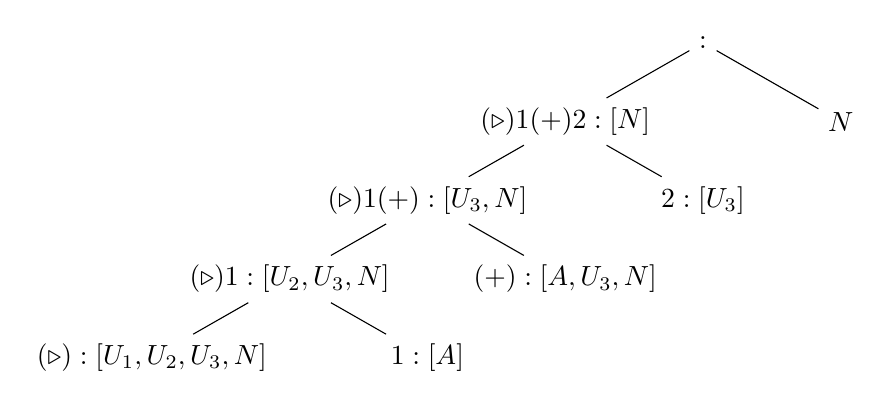
\begin{tikzpicture}
    \def\app{{\scriptsize app}}
    \def\f{{(\triangleright)}}
    \def\p{{(+)}}
    \node {:} [sibling distance = 3.5cm, level distance = 1cm]
        child {node {$\f 1 \p 2:[N]$}
            child {node {$\f 1 \p:[U_3, N]$}
                child {node {$\f 1:[U_2, U_3, N]$}
                    child {node {$\f: [U_1,U_2,U_3,N]$}}
                    child {node {$1: [A]$}}
                }
                child {node {$(+): [A,U_3,N]$}}
            }
            child {node {$2: [U_3]$}}
        }
        child {node {$N$}};
\end{tikzpicture}
}

We start with the elaboration of $(\triangleright) 1 (+) 2$ with the signature
requirement $[N]$ and the required type $N$.

\begin{itemize}
    \item The term is an application with the function term $(\triangleright) 1
        (+)$ and the argument $2$. We start the elaboration of the function term
        with the signature requirement $[U_3, N]$ and no required type.

    \item The term is again an application with the function term
        $(\triangleright) 1$ and the argument $(+)$. We start the elaboration
        of the function term with the signature requirement $[U_2, U_3, N]$ and
        no required type.

    \item The term is again an application with the function term
        $(\triangleright)$ and the argument $1$. We start the elaboration of the
        function term with the signature requirement $[U_1, U_2, U_3, N]$ and no
        required type.

    \item The term $(\triangleright)$ is a global name with the signature $[I,
        I, A, [A, P], P]$. Unification with the required signature $[U_1, U_2,
        U_3, N]$ results in
        $$
        \begin{array}{lll}
            U_1 &:=& A
            \\
            U_2 &:=& [A, U_3, N]
            \\
            P   &:=& [U_3, N]
        \end{array}
        $$
        Because of the two implicit arguments the term is elaborated as
        $(\triangleright)A P$ with the metavariables $A$ and $P$.

    \item Next the argument term $1$ has to be elaborated with the required
        signature $[A]$ and the required type $A$. This elaboration gets stuck
        on $A$, because the elaborator cannot decide the number type.

    \item Next the argument term $(+)$ is tried with the required signature $[A,
        U_3, N]$. The global name is ambiguous, but the ambiguity can be
        resolved by the result type. The signature is $[N, N, N]$. Unification
        with the required signature results in
        $$
        \begin{array}{lll}
            A &:=& N
            \\
            U_3 &:=& N
        \end{array}
        $$

    \item Now the complete term can be elaborated as
        $$
            (\triangleright) N (N \to N) \meta a (+) \meta b
        $$
        leaving the two holes $\meta a$ and $\meta b$ for the remaining
        arguments. However by unification the metavariables $\meta A$ and $\meta
        U_3$ are instantiated by $N$ and therefore the elaboration of the
        remaining arguments is unblocked and finally will succeed.
\end{itemize}


\end{document}
